\chapter{Results}\label{ch04:results}

This section presents the forecasting performance of SAMFormer, TimesFM, Time-MoE, TimeGPT, and regression baselines across different datasets (weather, finance, energy, and healthcare) and forecasting horizons. We evaluated the models using the root mean squared error (RMSE), the mean absolute error (MAE), and the coefficient of determination (R\textsuperscript{2}) to assess accuracy and reliability. Detailed metric breakdowns, including MAPE and explained variance, are provided in Appendix \ref{appendixA}. Moreover, Appendix \ref{appendixB} contains the predictions made by the models.

\section{Overall Model Performance Trends}

The transformer-based models, including \textbf{SAMFormer}, \textbf{TimesFM}, \textbf{Time-MoE}, and \textbf{TimeGPT}, generally outperform traditional regression baselines, particularly for longer forecasting horizons. Among them, \textbf{TimeGPT} demonstrates the lowest RMSE in short-term forecasting, making it highly effective for immediate predictions. However, its performance deteriorates as the forecasting horizon increases. \textbf{SAMFormer}, on the other hand, maintains stable performance across all datasets and horizons, proving to be the most consistent model. \textbf{Time-MoE} performs competitively in many cases but falls behind in certain domains, showing some variability in its effectiveness. \textbf{TimesFM}, however, struggles significantly, underperforming across multiple datasets, especially for longer forecasting horizons. In contrast, traditional regression models perform well for short-term forecasts but experience a noticeable decline in accuracy as the prediction horizon extends.

\begin{figure}[h]
    \centering
    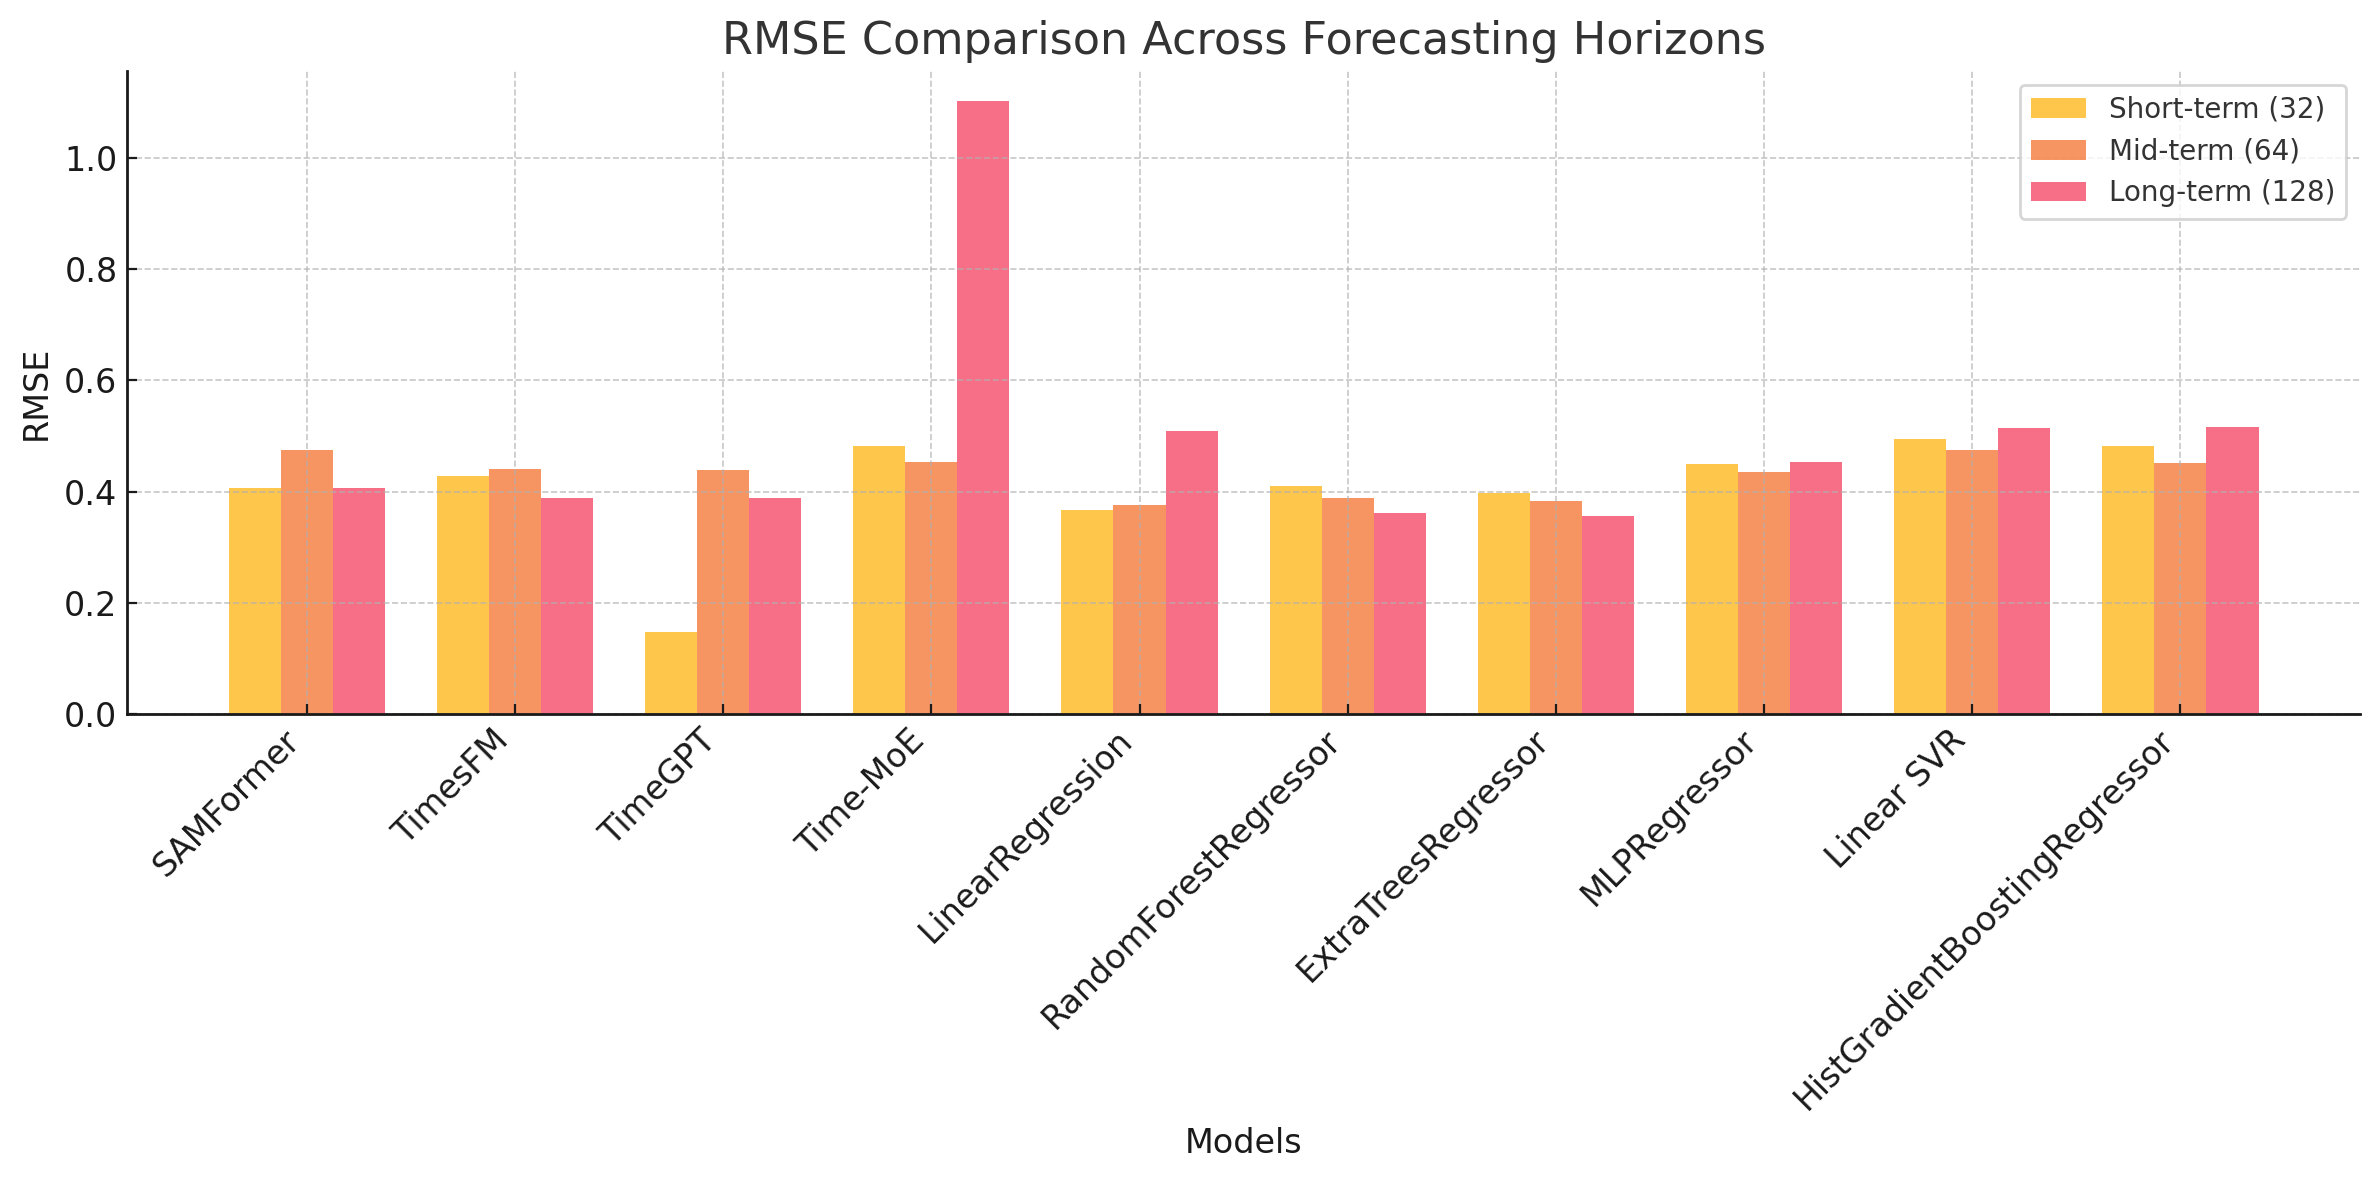
\includegraphics[width=\textwidth]{figures/performance across datasets.png}
    \caption{Performance Across Forecasting Horizons}
    \label{fig:performance_horizons}
\end{figure}

Full RMSE, MAE, and additional metric values are provided in \autoref{appendixA}.


\section{Performance Across Different Datasets}

\begin{figure}[h]
    \centering
    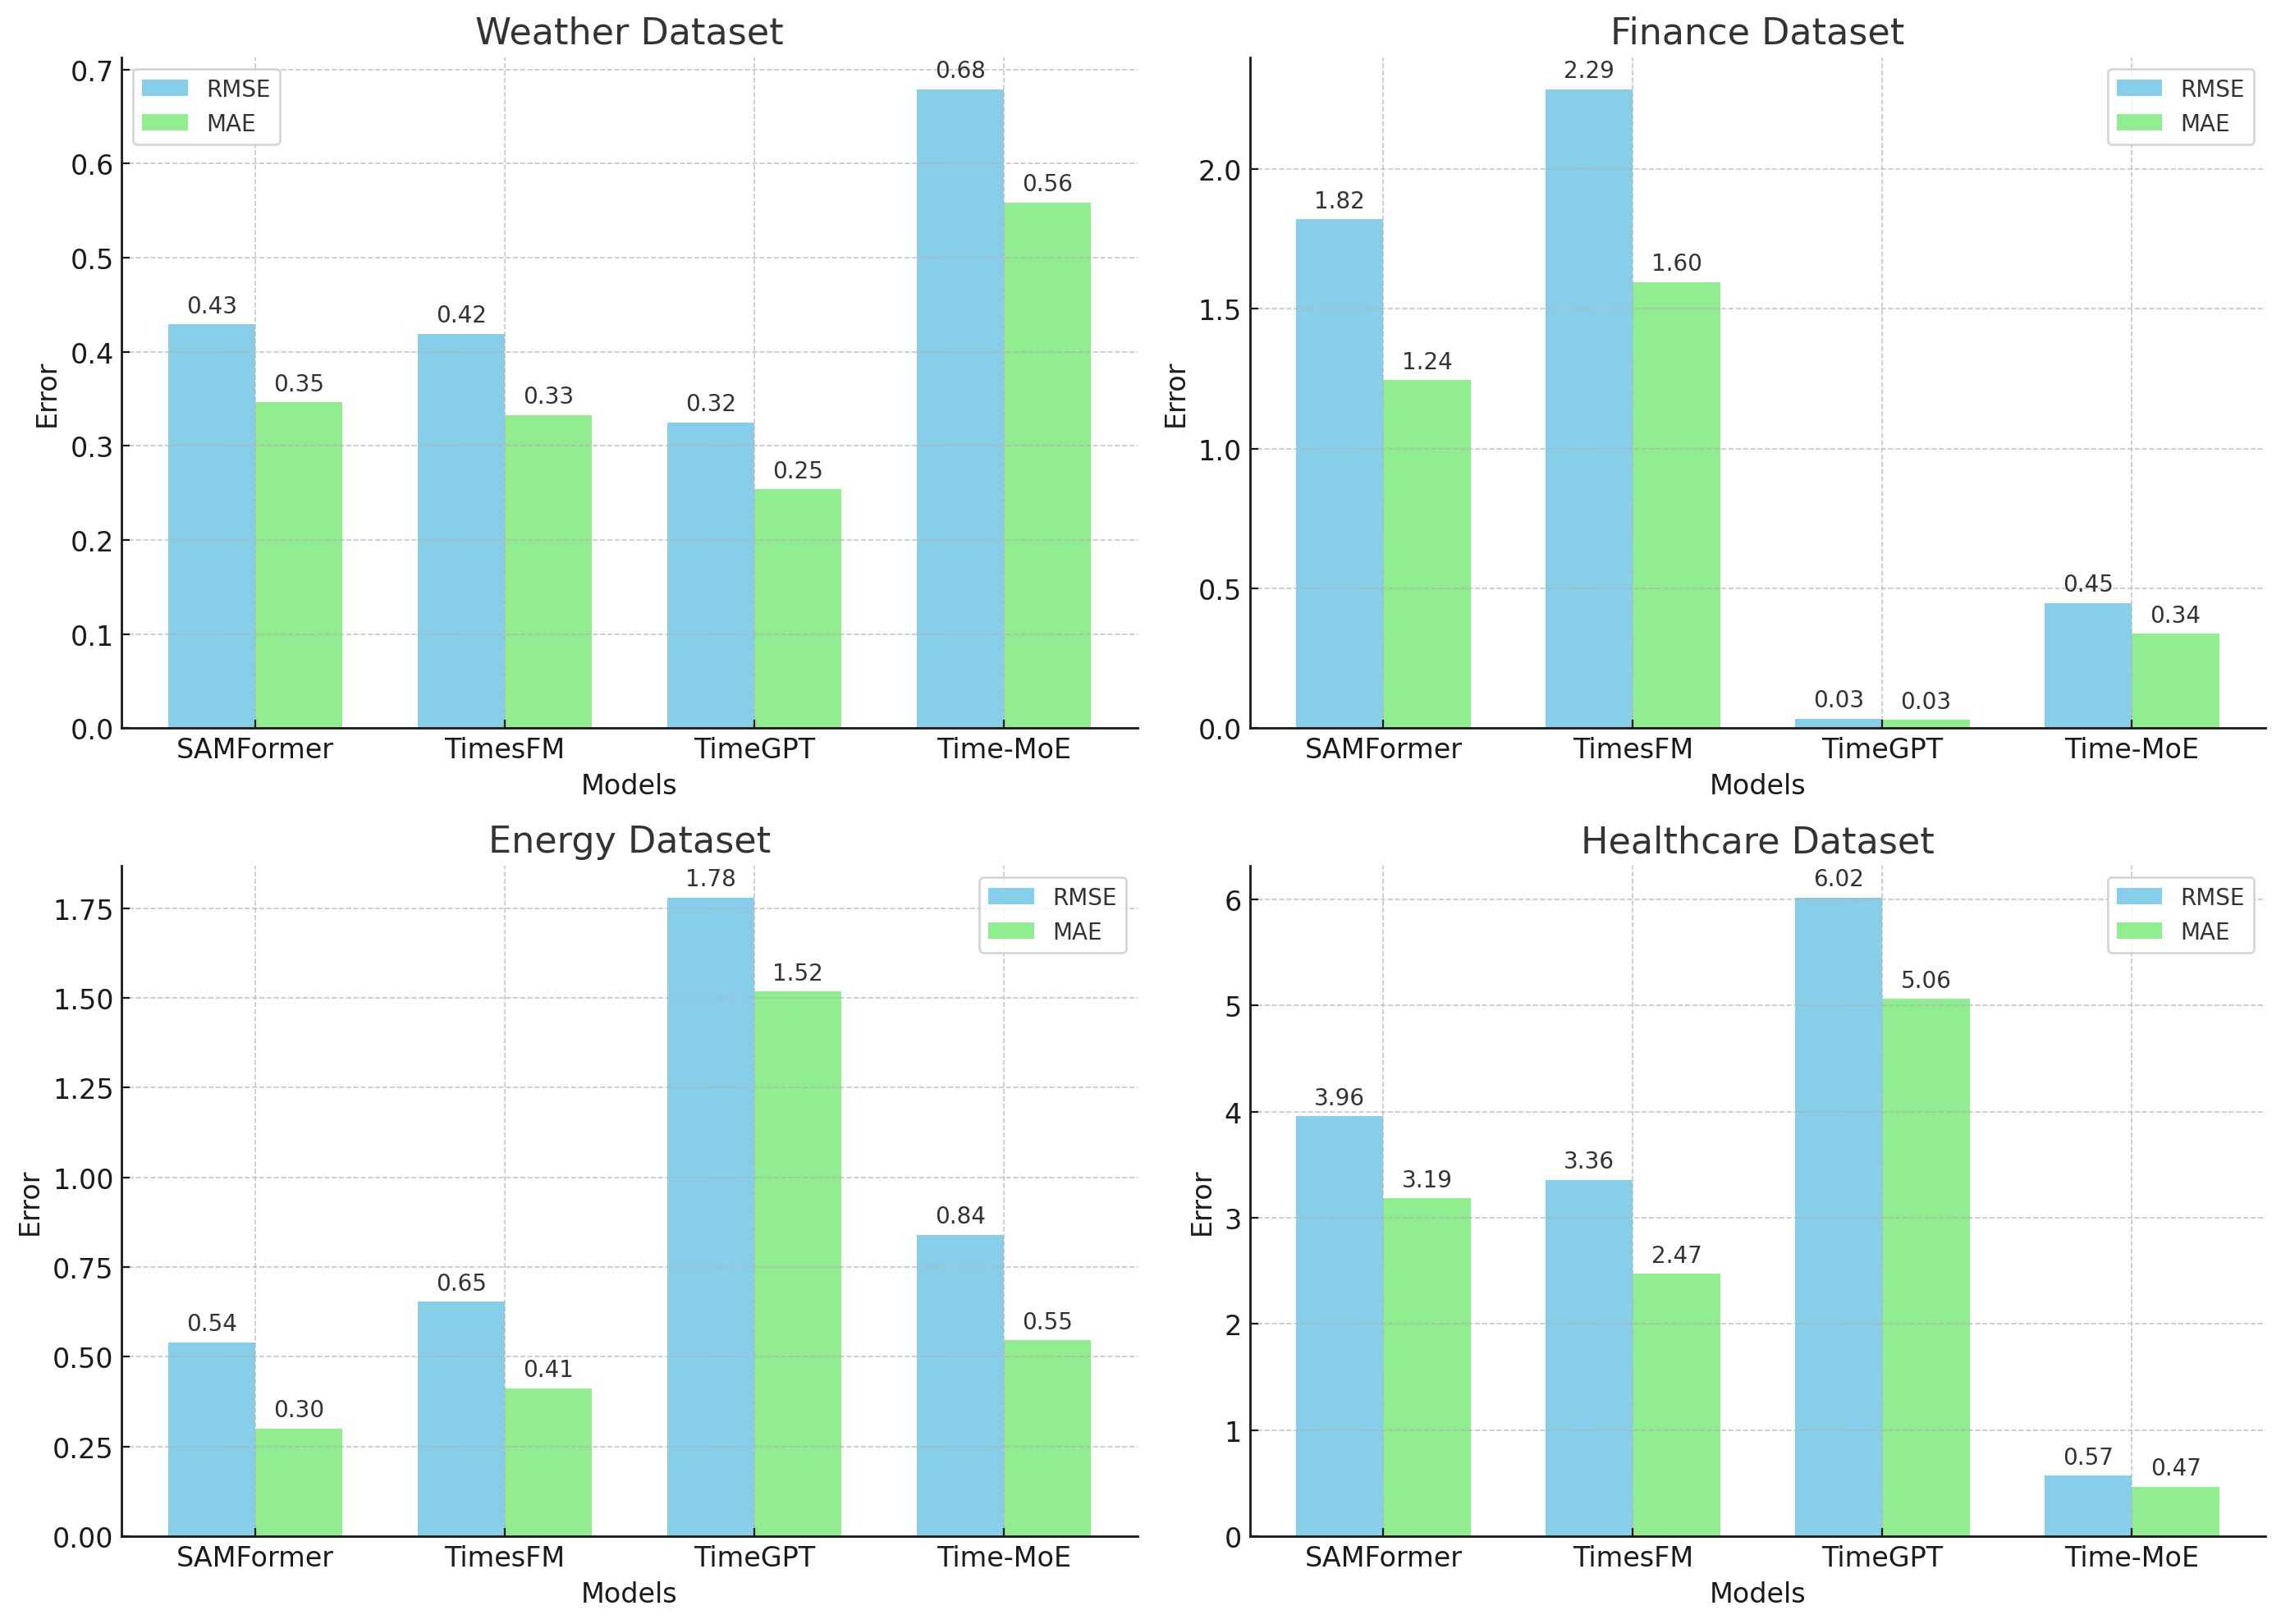
\includegraphics[width=\textwidth]{figures/models and datasets(1).png}
    \caption{Model Performance Across Datasets}
    \label{fig:performance_datasets}
\end{figure}



\subsection{Weather Forecasting}

For short-term weather forecasting, \textbf{TimeGPT} achieves the lowest RMSE at a horizon of 32, making it the most effective model for immediate predictions. Over longer forecasting horizons, \textbf{SAMFormer} proves to be the most stable, maintaining low RMSE and high R\textsuperscript{2} across all tested horizons. In contrast, \textbf{TimesFM} performs the worst, exhibiting significant errors and low R\textsuperscript{2} values, making it the least reliable model for weather forecasting.

\subsection{Financial Forecasting}

In financial forecasting, \textbf{SAMFormer} excels at long-term predictions, demonstrating superior accuracy and stability over extended horizons. Meanwhile, \textbf{TimeGPT} performs well in short-term stock price forecasting but struggles as the horizon length increases. \textbf{TimesFM} faces considerable difficulties in this domain, with errors surpassing those of even the baseline regression models. Traditional regression models exhibit high variance, leading to inconsistent and unreliable financial predictions.

\subsection{Energy Consumption Forecasting}

For energy consumption forecasting, \textbf{SAMFormer} achieves the lowest RMSE overall, particularly excelling in long-horizon forecasts. \textbf{TimeGPT} and \textbf{Time-MoE} also perform well, especially for mid-range forecasting horizons, though their accuracy diminishes as the horizon extends. Regression models show moderate performance but struggle significantly with longer horizons, highlighting their limitations in handling complex temporal dependencies in energy data.

\subsection{Healthcare Forecasting (COVID-19 Cases)}

In healthcare forecasting, specifically for COVID-19 case predictions, \textbf{SAMFormer} consistently outperforms other models, making it the most reliable choice for long-term forecasting. \textbf{TimeGPT} demonstrates reasonable accuracy in short-term forecasts but does not maintain its performance over extended horizons. Regression models, on the other hand, display erratic behavior, heavily influenced by fluctuations in case data, which makes them unreliable for healthcare forecasting.



\section{Impact of Forecasting Horizon Length}

Increasing the forecasting horizon from 32 to 128 steps generally results in reduced model accuracy across all datasets. Despite this decline, \textbf{SAMFormer} remains the most stable model, consistently maintaining competitive RMSE and high R\textsuperscript{2} values, even at longer horizons. \textbf{TimeGPT}, while excelling in short-term forecasting, experiences a noticeable drop in performance when extended to a horizon of 128. Traditional \textbf{regression models} exhibit the most significant deterioration, struggling to maintain accuracy as the forecasting horizon increases.

\begin{figure}[h!]
    \centering
    \begin{subfigure}{0.48\textwidth}
        \centering
        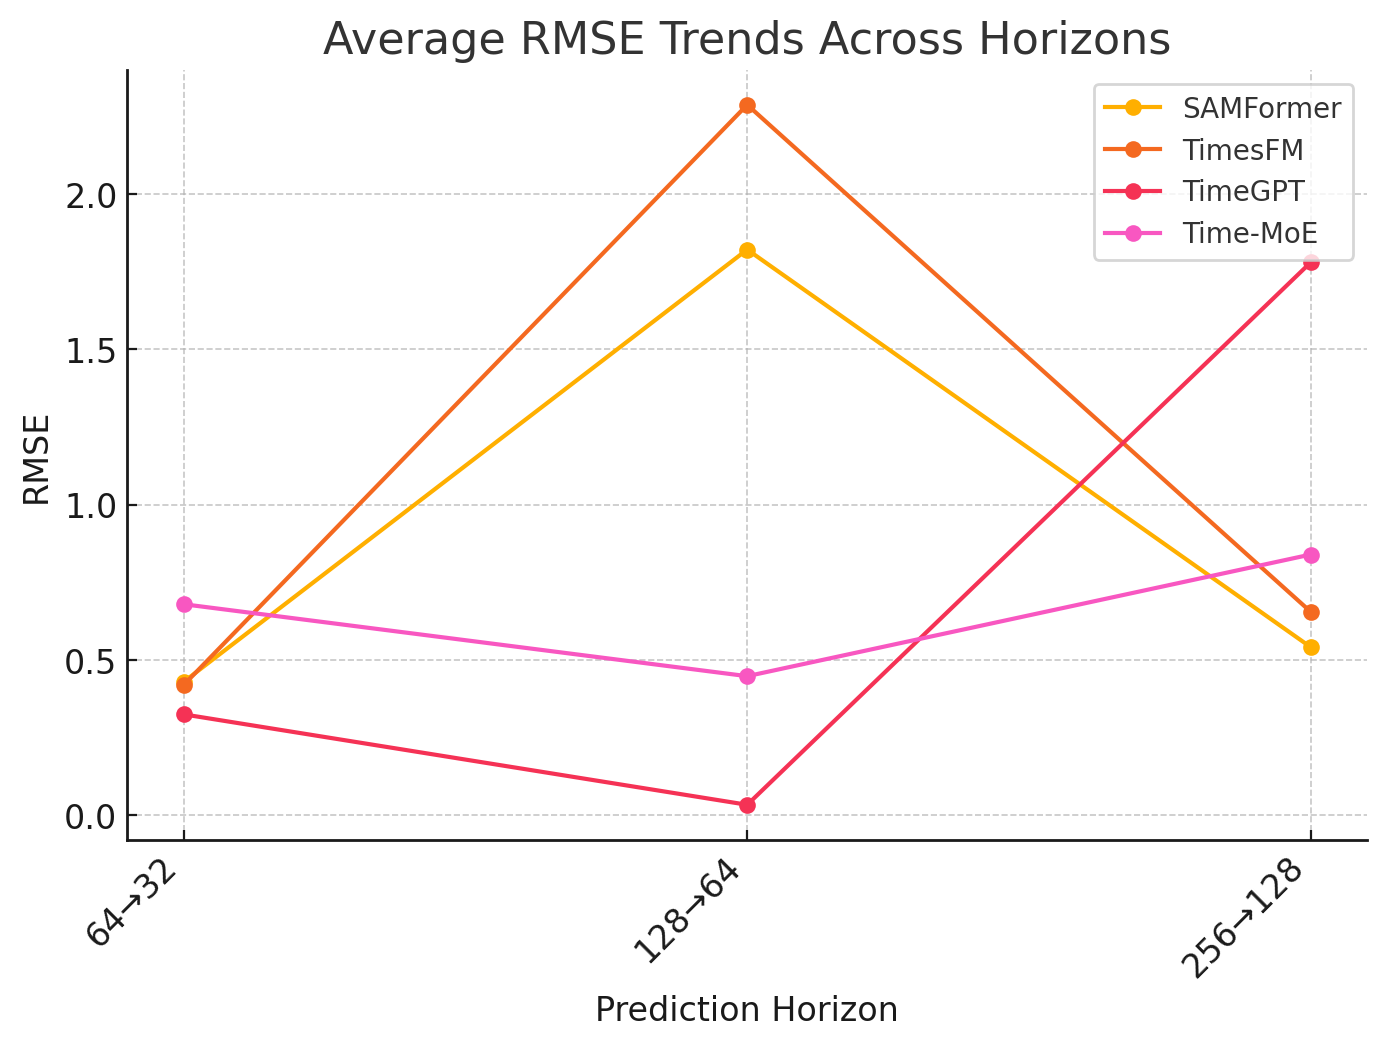
\includegraphics[width=\textwidth]{figures/rmse for horizons.png}
        \caption{RMSE Trends}
        \label{fig:rmse_trend}
    \end{subfigure}
    \hfill
    \begin{subfigure}{0.48\textwidth}
        \centering
        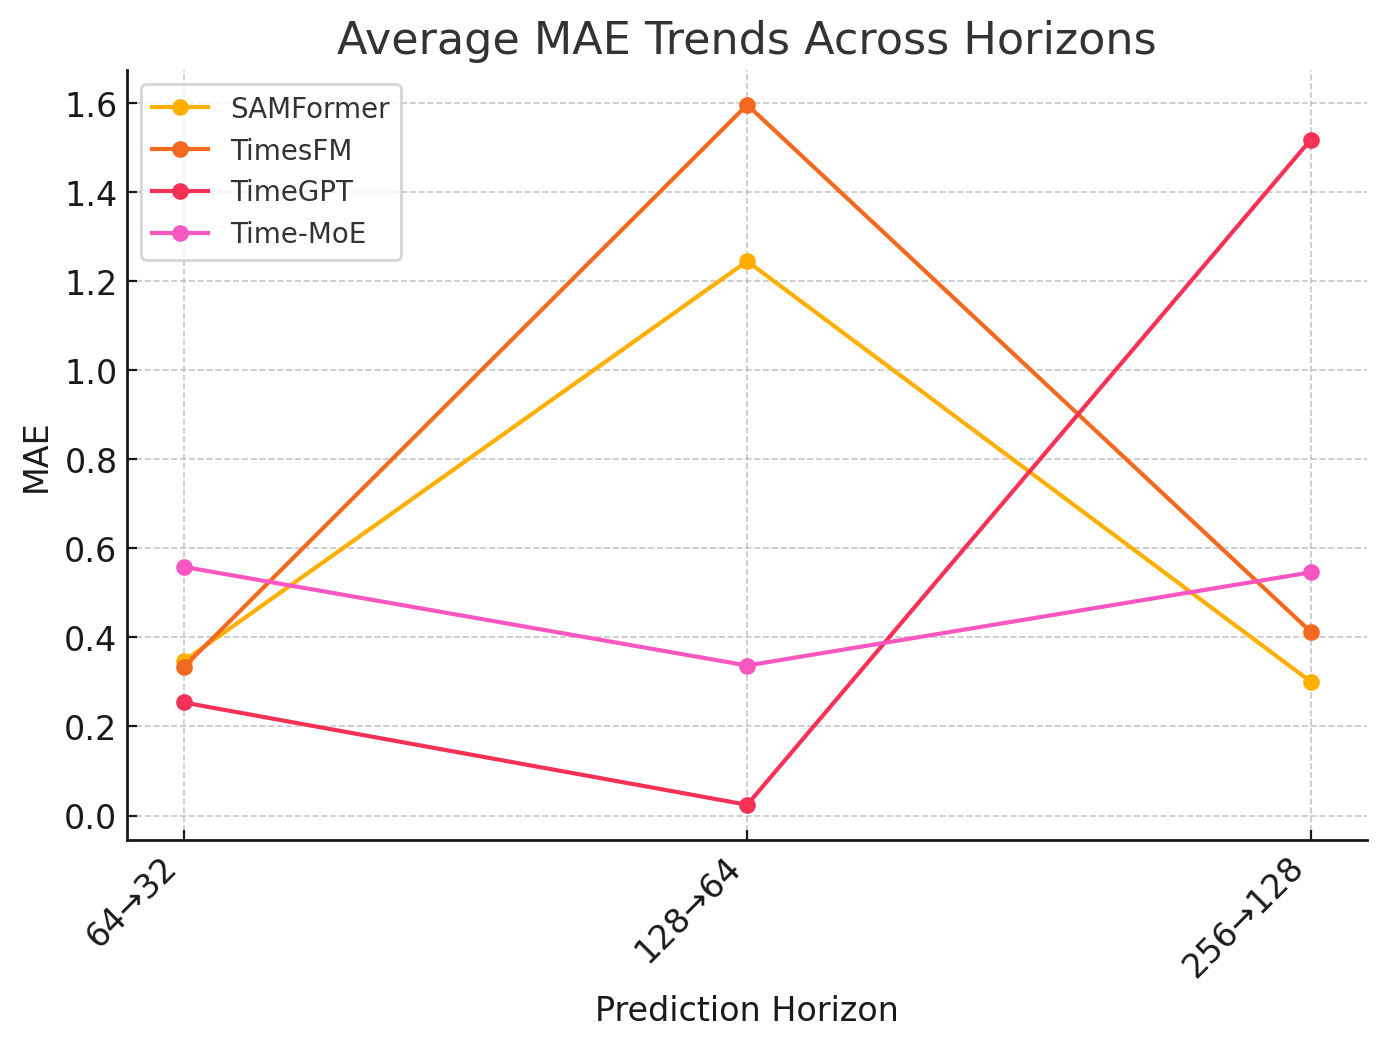
\includegraphics[width=\textwidth]{figures/mae for horizons.png}
        \caption{MAE Trends}
        \label{fig:mae_trend}
    \end{subfigure}
    \caption{Comparison of RMSE and MAE trends across different prediction horizons.}
    \label{fig:rmse_mae_comparison}
\end{figure}


\section{Comparison with Regression Baselines}

Traditional regression models, including \textbf{Linear Regression}, \textbf{Random Forest}, \textbf{Extra Trees}, and \textbf{MLP}, serve as baselines for comparison. Among these, \textbf{Linear Regression} performs well in short-term forecasts, particularly at a horizon of 32, but its accuracy declines significantly as the forecasting horizon extends. The most consistent regression model across different datasets is the \textbf{Extra Trees Regressor}, which maintains relatively stable performance. On the other hand, \textbf{Linear SVR} struggles the most, failing to capture nonlinear temporal trends effectively, making it the least reliable regression model in this evaluation.


\section{Fine-Tuning vs. Zeroshot Performance}

The impact of fine-tuning relative to zeroshot performance varies considerably across datasets and forecasting horizons, as well as by model.

For \textbf{Weather} forecasting, fine-tuning improves the performance of models like \textbf{TimeGPT} and \textbf{TimesFM} (e.g., TimeGPT achieves an RMSE of 0.1475 in fine-tuned mode versus 0.2045 in zeroshot for Horizon 32). However, the pre-trained \textbf{Time-MoE} model shows a much lower RMSE in the zeroshot setting (0.1300 for Horizon 32) than when fine-tuned (0.4824), suggesting that its pre-trained weights are already well-calibrated for short-term weather forecasting.

In the \textbf{Finance} domain, \textbf{TimeGPT} delivers nearly identical performance in both settings (e.g., RMSE around 0.0197 for Horizon 32), while \textbf{Time-MoE} and \textbf{TimesFM} exhibit only marginal differences between fine-tuned and zeroshot modes, with no clear overall advantage from fine-tuning.

For \textbf{Energy} forecasting, fine-tuning substantially benefits \textbf{TimesFM} (reducing its RMSE from approximately 1.1627 in zeroshot mode to 0.5790 in fine-tuned mode). In contrast, \textbf{TimeGPT} shows slightly better performance in the zeroshot setting, and \textbf{Time-MoE} performs comparably in both modes.

Finally, in \textbf{Healthcare} forecasting, all models tend to achieve lower forecasting errors in the zeroshot configuration. For instance, \textbf{TimeGPT} has an RMSE of 0.7071 in zeroshot mode compared to 2.9776 when fine-tuned. Similarly, both \textbf{Time-MoE} and \textbf{TimesFM} yield lower errors in their zeroshot versions, indicating that additional fine-tuning may not be beneficial for these models in healthcare tasks.

The varying explained variance scores (see Appendix \ref{appendixA}) highlight the varying impact of fine-tuning across models and domains. Fine-tuning improved \textbf{TimeGPT} and \textbf{TimesFM} in weather forecasting but had little effect in finance, where zeroshot models performed similarly. In healthcare, zeroshot models often had higher explained variance, suggesting that fine-tuning may introduce overfitting rather than improving generalization.

\begin{figure}[ht]
    \centering
    \begin{minipage}{0.32\textwidth}
        \centering
        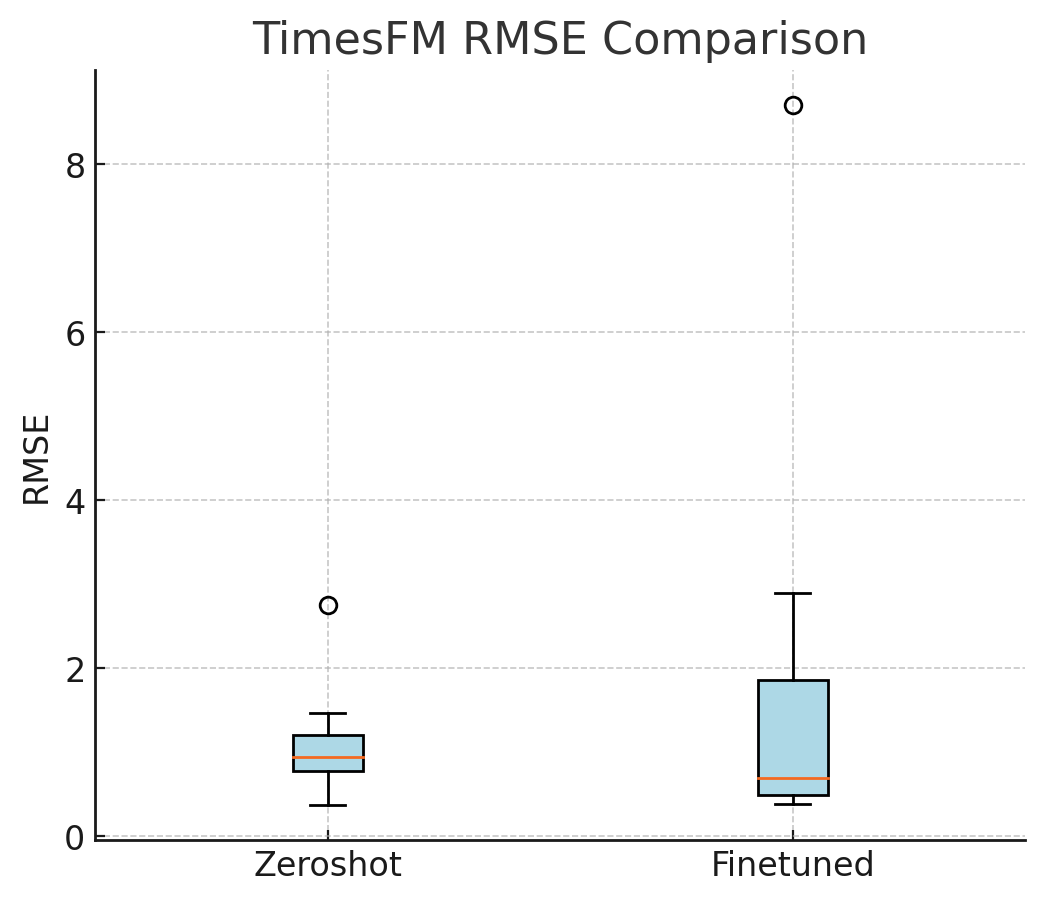
\includegraphics[width=\textwidth]{figures/timesfm rmse comparison.png}
    \end{minipage}
    \begin{minipage}{0.32\textwidth}
        \centering
        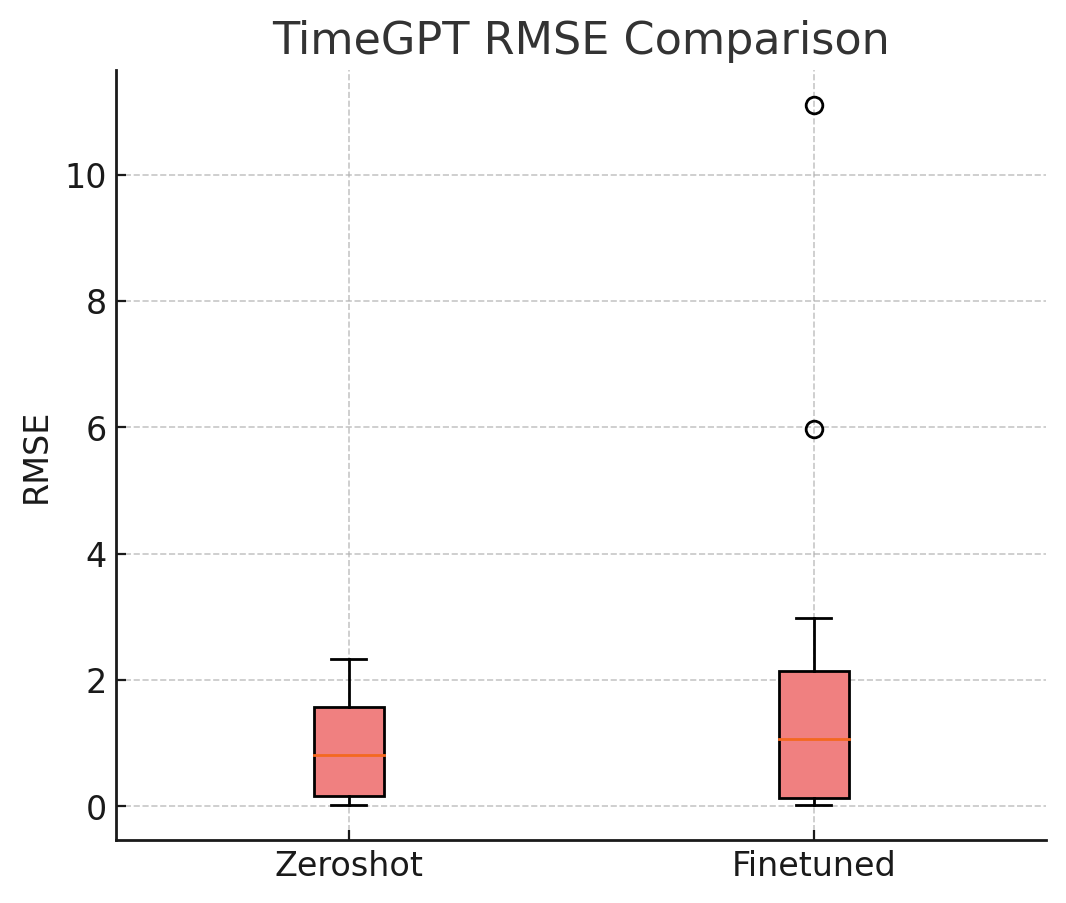
\includegraphics[width=\textwidth]{figures/timegpt rmse comparison.png}
    \end{minipage}
    \begin{minipage}{0.32\textwidth}
        \centering
        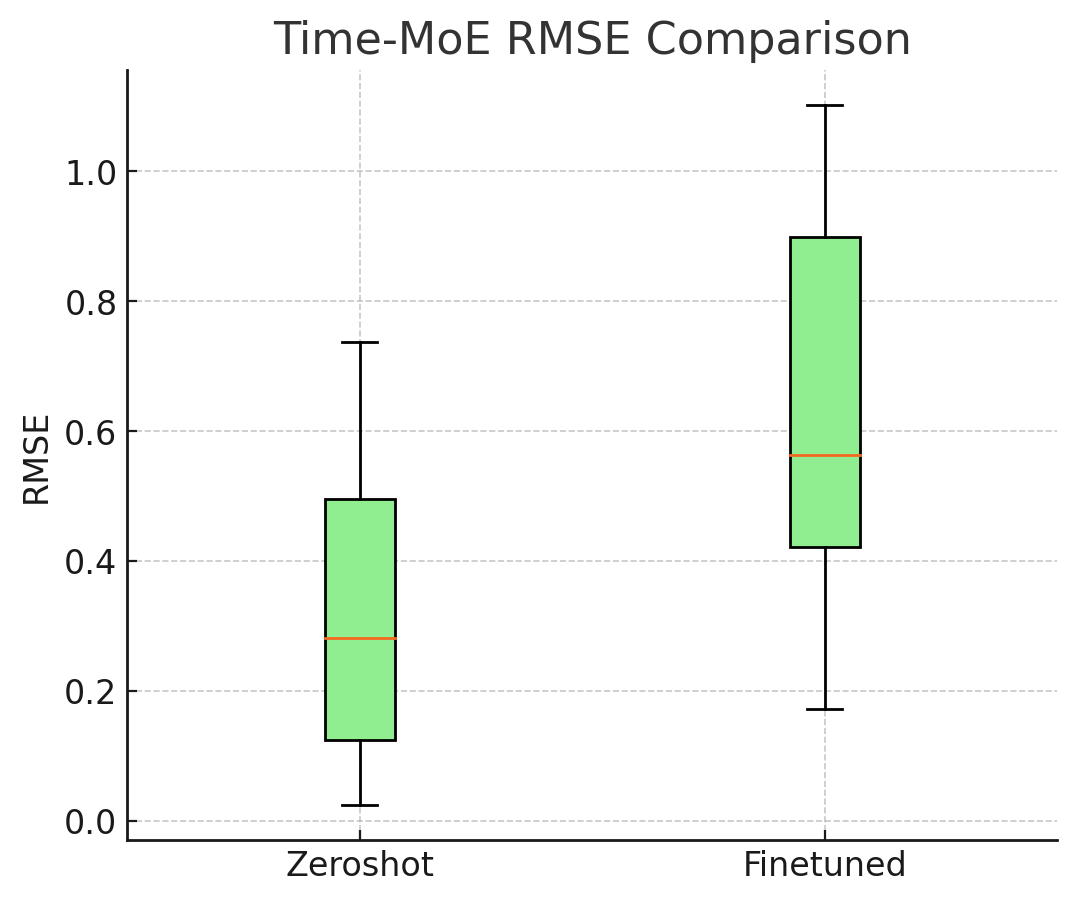
\includegraphics[width=\textwidth]{figures/time-moe rmse comparison.png}
    \end{minipage}
    \caption{RMSE comparison of TimesFM, TimeGPT, and Time-MoE models.}
    \label{fig:three_placeholders}
\end{figure}


Overall, while fine-tuning can yield improvements—most notably for \textbf{TimeGPT} in weather and energy forecasting and for \textbf{TimesFM} in energy forecasting—the advantages of fine-tuning are not uniform across all models and datasets. In several cases, particularly in finance and healthcare, the zeroshot performance is competitive or even superior. In the case of Time-MoE, finetuning did not yield any apparent performance increases.